\documentclass[12pt]{article}
\usepackage{hyperref}
\usepackage{graphicx}
\usepackage[font=small,labelfont=bf]{caption}
\title{Analisi sito}
\date{}
\author{Alessio Luca}
\begin{document}
\pagenumbering{arabic}



\begin{titlepage}

\newcommand{\HRule}{\rule{\linewidth}{0.5mm}} % Defines a new command for the horizontal lines, change thickness here

\center % Center everything on the page
 
%----------------------------------------------------------------------------------------
%	HEADING SECTIONS
%----------------------------------------------------------------------------------------

\textsc{\LARGE Universit\`a degli Studi di Padova}\\[1.5cm] % Name of your university/college
\textsc{\Large Laurea in Informatica}\\[0.5cm] % Major heading such as course name
\textsc{\large Corso di Tecnlogie Web 2}\\[0.5cm] % Minor heading such as course title

%----------------------------------------------------------------------------------------
%	TITLE SECTION
%----------------------------------------------------------------------------------------

\HRule \\[0.4cm]
{ \huge  Progetto di fine corso}\\[0.3cm] % Title of your document
\HRule \\[1.5cm]
 
%----------------------------------------------------------------------------------------
%	AUTHOR SECTION
%----------------------------------------------------------------------------------------

\begin{minipage}{0.4\textwidth}
\begin{flushleft} \large
\emph{Studente:}\\
Luca \textsc{Alessio} % Your name
\end{flushleft}
\end{minipage}
~
\begin{minipage}{0.4\textwidth}
\begin{flushright} \large
\emph{Matricola:} \\
\textsc{1070690} % Supervisor's Name
\end{flushright}
\end{minipage}\\[4cm]

% If you don't want a supervisor, uncomment the two lines below and remove the section above
%\Large \emph{Author:}\\
%John \textsc{Smith}\\[3cm] % Your name

%----------------------------------------------------------------------------------------
%	DATE SECTION
%----------------------------------------------------------------------------------------

{\large 20/03/2016}\\[3cm] % Date, change the \today to a set date if you want to be precise

%----------------------------------------------------------------------------------------
%	LOGO SECTION
%----------------------------------------------------------------------------------------

%\includegraphics{Logo}\\[1cm] % Include a department/university logo - this will require the graphicx package
 
%----------------------------------------------------------------------------------------

\vfill % Fill the rest of the page with whitespace

\end{titlepage}

\newpage
\renewcommand{\contentsname}{Indice}
\tableofcontents

\newpage
\pagenumbering{arabic}

\section{Una breve introduzione}
\subsection{Cos'\`e Reddit?}
\begin{itemize}
	\item Il sito si autodefinisce come "a source for what's new and popular on the Internet".
	\item All'interno di Reddit gli utenti registrati possono pubblicare post testuali e condividere contenuti esterni
	\item Gli utenti hanno poi la possibilit\`a di valutare un contenuto (con un +1 o un -1) e di discuterlo attraverso un sistema di commenti a cascata
	\item Reddit \`e una community formata da molteplici sotto-community ("subreddits"), ogni subreddit tratta un argomento specifico e raggruppa i post inerenti a quell'argomento
	\item Attraverso il proprio voto gli utenti determinano quali contenuti verranno evidenziati in ciascun subreddit e, per riflesso, nella home page principale del sito
\end{itemize}

\subsection{Guida basilare alla struttura del sito}
La pagina principale di Reddit \`e accessibile dall'indirizzo \url{www.reddit.com}, abbreviazione di \url{www.reddit.com/r/all} , da qui si pu\`o avere una panoramica di tutto ci\`o che al momento \`e popolare tra gli utenti del sito.\\
Se voglio accedere ad informazioni su un preciso argomento mi baster\`a entrare nel relativo subreddit (se esistente), posso fare ci\`o attraverso un link oppure usando la sintassi universale:\\ \centerline{reddit.com/r/namesubreddit(/path-to-specific-content)}\\ Se ad esempio sto cercando notizie riguardanti il mondo del cinema andr\`o su /r/movies, se cerco notizie sulla realt\`a nostrana visiter\`o /r/italy, se voglio discutere con altri appassionati di Batman andr\`o su /r/batman e cos\`\i\  via.\\ \\
Il motto del sito \`e "There is a subreddit for everything!".
\\ \\ \textbf{N.B. Questa analisi di usabilit\`a \`e stata redatta nel periodo di fine marzo / inizio aprile 2016, eventuali contenuti del sito potrebbero essere cambiati nel tempo.}

\newpage
\section{Analisi di usabilit\`a della homepage} %rivedere suddivisone in paragrafi
%suddivire sezioni principali: sito normale, utenti registrati, subreddit, parte mobile
\subsection{Analisi del dominio}
Reddit, unione delle parole read ed edit, \`e un nome corto e semplice da memorizzare per l'utenza media.
Il sistema di sub-redditing e la sintassi di dominio corrispondente diventano pratici con l'uso per un utente esperto ma sono poco intuitivi per un utente che si affaccia alla piattaforma per la prima volta. Esploreremo meglio questo aspetto pi\`u avanti.

\subsection{A prima vista}
Per prima cosa cercheremo di analizzare la pagina principale tramite gli occhi di un utente che visita il sito per la prima volta: capisce dove si trova? Capisce dov'\`e quello che cerca? Vediamo se le 6 W vengono soddisfatte.
\begin{figure}[ht!]
\centering

\includegraphics[width=90mm]{home1}
\caption{vedi file home1.jpg}
\end{figure}
%inserire foto
\subsubsection{What} Cosa trovo in questo sito? A prima vista l'utente medio si trova spiazzato davanti alla home di Reddit. Ho chiesto ad un amico (che non conosceva Reddit) di entrare nel sito e darmi il suo parere a caldo, queste sono state alcune delle sue reazioni:
\begin{itemize}
	\item\textit{"Cosa trovo in questo sito? Pare un po' di tutto, ma i contenuti sembrano messi a caso"}
	\item \textit{"Dov'\`e la parte interessante?"} \\L'occhio si perde, niente di particolare cattura l'attenzione dell'utente che comincia a scrollare. \\\textit{"Ma \`e tutto uguale?"}
	\item \textit{"Devo dire che \`e bruttino questo sito, l'hai fatto tu?"} \\Il CSS \`e un po' troppo minimale e poco colorato, cosa che non tutta l'utenza gradisce, anche questo aspetto pu\`o impattare i timer di permanenza.
	\item \textit{"Credo sia una via di mezzo tra un forum e un blog (?) solo che ancora non capisco di cosa tratta"} \\L'utente dopo un po' (se non ha abbandonato la pagina) comincia a farsi un'idea del sito, a questo punto chiedo al mio amico di spiegarmi secondo lui come funziona.
	\item \textit{"Allora, siamo nella sezione "popolari" della home o almeno cosi \`e scritto qua in alto, queste sotto dovrebbero essere le cose popolari} (prova a visitare vari post e capisce un po' come funziona)\textit{, ok, hmmm, un po' di pubblicit\`a, un disegnino, invia link, invia messaggio, questi credo servano a postare cose nel sito, almeno sembrano cose inserite dagli utenti; sopra c'\`e la registrazione quindi penso ti serva un account, in cima a bordo pagina c'\`e un menu? cos'\`e?} (apre un po' di subreddit e comincia a capire come \`e strutturato il sito)\textit{ ah ok praticamente se voglio vedere cose che riguardano un certo argomento vado nella pagina corrispondente che le raccoglie e qua nella home ne mostrano un po' a caso per incuriosirti immagino... poi qui, vicino ai link c'\`e un numero con delle frecce che penso servano per dare mi piace o non mi piace, si pu\`o commentare e condividere anche se potevano scriverlo un po' pi\`u grande, ah e qua} (indica il link al subreddit del contenuto postato)\textit{ in caratteri inleggibili c'\`e tipo il link alla sotto pagina con altre cose riguardanti lo stesso argomento... ah e qua in fondo alla pagina ci sono info e aiuto che immagino ti spieghino tutto e che forse dovevo leggere prima ma non le ho viste..."}
\end{itemize}
In conclusione, l'utente medio \`e inizialmente spaesato e pi\`u propenso ad abbandonare il sito che a restarci, ma se continua ad esplorarlo capisce man mano il suo funzionamento.
\newpage
\subsubsection{Where} Siamo nella pagina principale e questa informazione \`e evidenziata dal sotto-men\`u in cima alla pagina. Reddit \`e un sito che si dirama molto "orizzontalmente" in vari subreddits ma ciascun subreddit ha una diramazione verticale praticamente nulla (un subreddit linka a vari post ma i post in s\`e non linkano ad altre pagine interne) per cui il sito non necessit\`a di breadcrumb particolarmente dettagliati. \\Per gli utenti abituali il men\`u in alto \`e molto comodo e compatto.
\\

\subsubsection{Why} Perch\`e dovrei cercare le informazioni che mi interessano su Reddit e non altrove? Reddit \`e un sito sia per chi cerca qualcosa in particolare sia per chi sta navigando senza un obiettivo: un utente che sta cercando informazioni su di un determinato argomento indirizzer\`a le proprie ricerche verso il subreddit che tratta quell'argomento dove potr\`a trovare anche notizie, approfondimenti e discussioni collegate mentre, un utente che sta visitando il sito per svago senza uno scopo preciso, quasi sicuramente trover\`a qualcosa di nuovo che lo intrattenga.
\\
\subsubsection{How} Come navigo in questo sito? Come visto nel punto What, la navigazione appare inizialmente confusa ma man mano che l'utente esplora il sito comincia ad apprenderne le meccaniche. Sono presenti varie opzioni di classificazione dei contenuti (sort per data, punteggio eccetera). La barra di ricerca si trova in una posizione standard (in alto a destra come la maggior parte dei siti) ed \`e ampia all'incirca 33 caratteri (sotto i 30 causa frustrazione all'utente). Quando l'utente effettua una ricerca, che per default copre interamente il sito, pu\`o inoltre specificare degli intervalli di restrizione (punteggio, subreddit, data eccetera) da applicare sulla visualizzazione dei risultati.
\\
\subsubsection{When} Novit\`a del sito? Il sito presenta un contenuto dinamico nella home che cambia continuamente. Alcuni eventi importanti organizzati da Reddit, come AMA (Ask Me Anything) di persone famose o iniziative di beneficenza, sono molto promossi e vengono molto pubblicizzati, spesso infatti
 vanno proprio a sostituire i banner pubblicitari (vedi sezione Pubblicit\`a).
\\
\subsubsection{Who} Il logo \`e presente in alto a sinistra (anche se un po' piccolo) e consiste nella scritta "reddit" affiancata da un esserino bianco, la mascotte del sito. Come Google a volte il logo cambia durante occorrenze particolari. Chi o cosa c'\`e dietro a Reddit? E' tutto spiegato nelle FAQ (che potevano anche essere linkate in un posto un po' pi\`u visibile). A fondo pagina, oltre alle FAQ, sono presenti vari link che conducono a pagine di spiegazione sulle funzionalit\`a del sito e sulle sue origini.
\newpage
\subsection{Altri elementi nella pagina}
\begin{figure}[ht!]
\centering

\includegraphics[width=90mm]{home2}
\caption{vedi file home2.png}
\end{figure}
Il sito adotta una semplice struttura a pannelli: un pannello superiore (header), due pannelli centrali (uno dedicato al men\`u di navigazione a l'altro al contenuto) e un pannello inferiore (footer). \\A differenza della maggior parte dei siti, dove il sotto-pannello centrale che funge da "nav" \`e situato a sinistra, qui il "nav" si trova sul lato destro dello schermo mentre i contenuti vengono presentati sulla sinistra. Questa scelta strutturale fa in modo che l'attenzione dell'utente (che ricordiamo effettua una scansione della pagina ad "F" prediligendo ovvero il lato sinistro dello schermo) sia da subito rivolta al contenuto vero e proprio della pagina in modo tale da fornire subito l'informazione cercata allungando di conseguenza i timer di permanenza dell'utente nel sito.

\subsection{Pubblicit\`a} %spostare in cima
Nella maggior parte delle pagine di Reddit la pubblicit\`a \`e praticamente assente o ridotta ad uno o due banner (che spesso pubblicizzano altri subreddit o eventi tenuti da Reddit), ci\`o \`e dovuto all'alto finanziamento ricevuto dalla community tramite l'iniziativa Reddit Gold, non approfondir\`o questo aspetto perch\`e esula dall'analisi del sito ma \`e spiegato nelle FAQ nel footer. In ogni caso i banner sono sempre statici (il che \`e positivo) ed alcuni possono anche essere chiusi. Non sono presenti pop-up tranne in alcune occasioni particolari quali messaggi d'errore (es. "non puoi commentare, devi prima creare un account"). Durante la prima navigazione nel sito compare in basso un banner dei cookie, anche se risalta poco ed \`e situato in una zona fredda potrebbe comunque dare fastidio ad alcuni utenti.

\newpage

\section{Analisi homepage per utenti loggati}
Quando ad accedervi \`e un utente registrato la pagina principale del sito si presenta leggermente differente: \\
\begin{figure}[ht!]
\centering

\includegraphics[width=90mm]{myhome}
\caption{vedi file myhome.png}
\end{figure} \\
non viene pi\`u visualizzato /r/all ma un insieme di post tratti dai subreddit preferiti dell'utente (di questo parleremo in una sezione successiva), il pannello di destra cambia leggermente (scompare il modulo di iscrizione, si aggiunge il tasto "crea subreddit") e viene aggiunta una semicolonna a scomparsa sulla sinistra dello schermo. Questo elemento aggiuntivo ha lo scopo di aiutare l'utente nell'esplorazione proponendogli contenuti non ancora visitati e altre feature minori del sito come ad esempio la possibilit\`a di fare il merge di pi\`u subreddit. \\ \\ Cliccando sui pulsanti per il submit di nuovi contenuti l'utente verr\`a indirizzato ad una pagina contenente un form: \\
\begin{figure}[ht!]
\centering
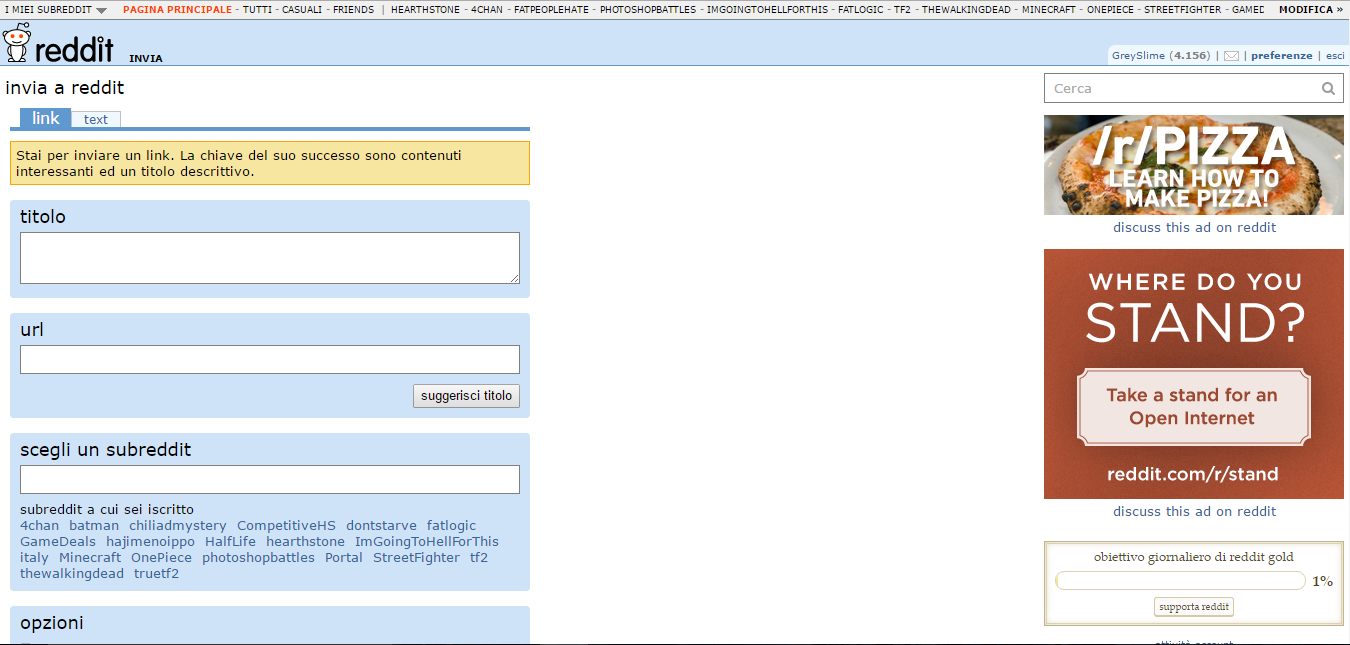
\includegraphics[width=90mm]{submit}
\caption{vedi file submit.png}
\end{figure} \\
il form \`e molto semplice, un campo per il titolo del post, un campo per il contenuto (che pu\`o essere un link ad un sito esterno oppure del testo nel caso l'utente voglia iniziare una discussione) e un campo in cui viene richiesto di specificare il subreddit dove il post verr\`a pubblicato; nulla da criticare in questa pagina, \`e molto semplice e comprensibile, per il resto ricalca la home.
\\
\section{La pagina profilo utente}
L'utente ha la possibilit\`a di visitare la propria pagina personale sempliemente cliccando sul proprio nome in alto a destra da qualsiasi pagina di Reddit. \\
\begin{figure}[ht!]
\centering

\includegraphics[width=90mm]{myprofile}
\caption{vedi file myprofile.png}
\end{figure} \\
In questa pagina l'utente potr\`a visualizzare varie informazioni come la cronologia dei post inviati, i post valutati positivamente o negativamente, i commenti lasciati in passato, post salvati da leggere pi\`u tardi e qualche statistica come il punteggio in "karma" dell'utente.\\ Ogni utente di Reddit ha un punteggio "karma" che viene calcolato sommando le valutazioni positive e negative che gli altri utenti hanno espresso sui contenuti che abbiamo pubblicato e sui commenti che abbiamo lasciato dal momento della nostra iscrizione sino ad oggi. L'utente pu\`o selezionare quale tipo di cronologia visualizzare tramite il semplice men\`u a schede posto sotto l'header.\\ \\Nel complesso questa pagina resta minimale come il resto del sito e abbastanza semplice da comprendere, non vedo perci\`o pecche da segnalare. L'utente pu\`o visitare anche i profili degli altri utenti semplicemente cliccandone sul nome, in tal caso verr\`a indirizzato ad una pagina analoga a quella personale. 

\section{Analisi subreddit interni}
Come gi\`a accennato, con il termine subreddit si denota un forum dedicato ad un topic specifico all'interno del sito principale Reddit, una sorta di "sito dentro al sito". Ma come \`e strutturato un subreddit? Cosa differenzia i vari subreddit fra loro? Vediamo qualche esempio... \\ \\Nelle seguenti immagini si possono osservare tre differenti subreddit: /r/web\_design (un subreddit di discussione per appassionati del settore web),
\\
\begin{figure}[ht!]
\centering
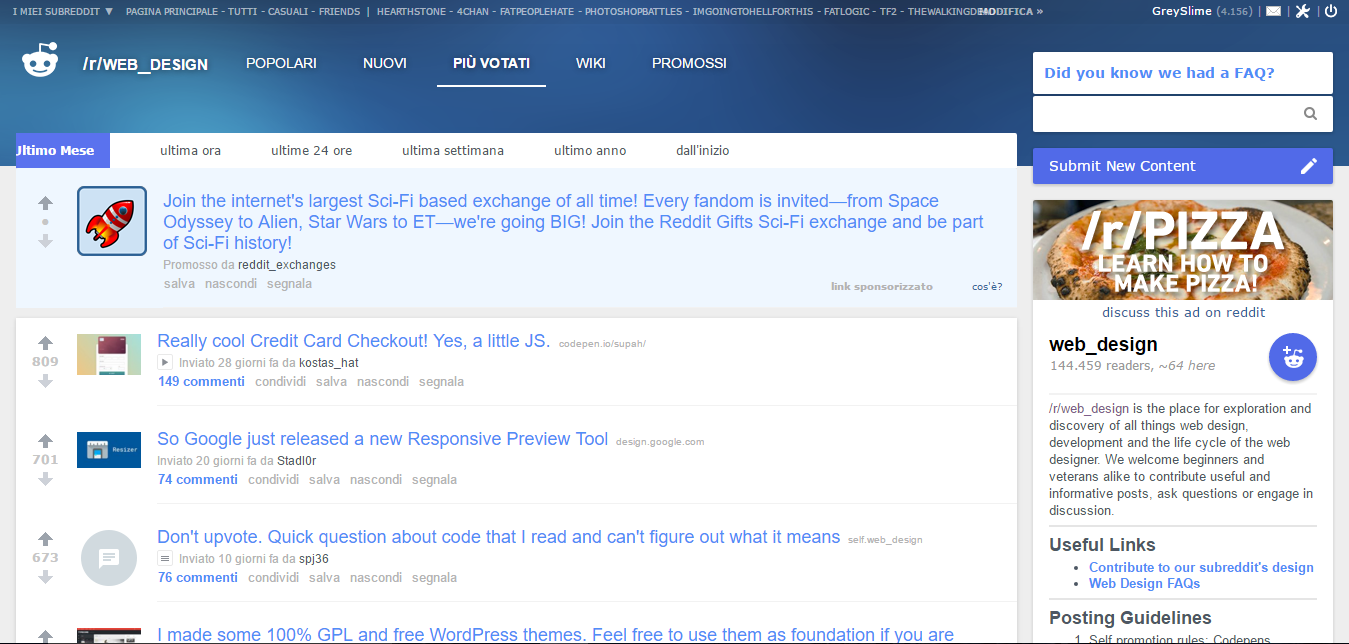
\includegraphics[width=90mm]{webdesign}
\caption{vedi file webdesign.png}
\end{figure} 
\\ \\
 /r/italy (un subreddit di ritrovo per utenti nostrani o per turisti in cerca di informazioni sulla nostra penisola)
\\
\begin{figure}[ht!]
\centering
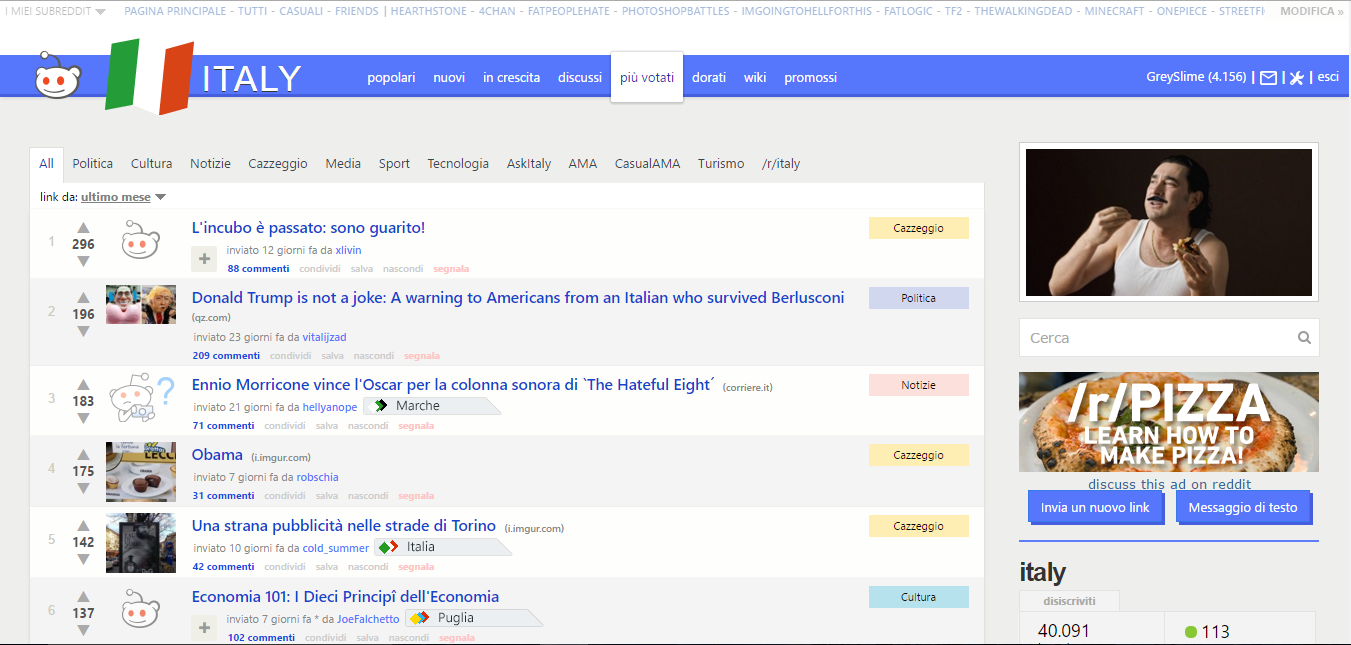
\includegraphics[width=90mm]{italy}
\caption{vedi file italy.png}
\end{figure} 
\newpage
ed /r/thewalkingdead (subreddit frequentato da appassionati della serie tv/fumetto "The Walking Dead").
\\
\begin{figure}[ht!]
\centering

\includegraphics[width=90mm]{twd}
\caption{vedi file twd.png}
\end{figure} 
\\ \\
Come si pu\`o notare dalle immagini, il template adottato da ogni subreddit \`e lo stesso e ricalca quello a pannelli della pagina principale, l'unica cosa a cambiare \`e il css, per i sei assi dell'informazione valgono quindi le stesse osservazioni fatte sulla home. \\Il pannello sulla destra contiene per\`o molte altre informazioni come le regole del subreddit, annunci dei moderatori, calendario degli eventi in arrivo e altro, il contenuto varia da subreddit a subreddit e pu\`o essere pi\`u o meno lungo portando a volte anche ad un eccessiva distorsione della pagina come si pu\`o notare ad esempio su \href{www.reddit.com/r/thewalkingdead}{/r/thewalkingdead}.\\ Nelle immagini precedenti ci\`o non si nota per motivi di spazio ma si pu\`o verificare di persona navigando nel sito. In casi del genere sarebbe meglio delegare la spiegazione delle regole/annunci/altro ad altre pagine interne al sito e nella pagina principale del subreddit lasciare solo un elenco di link a queste ultime. \\Questo fenomeno non \`e presente in tutti i subreddit (si veda infatti \href{www.reddit.com/r/web_design}{/r/web\_design} dove la barra laterale \`e molto pi\`u pulita), ma li dove accade andrebbe corretto. \\ \\L'utente ha la possibilit\`a di "iscriversi" ad un subreddit cliccando sul pulsante apposito (situato solitamente vicino al tasto per submittare nuovi contenuti), cos\`i\  facendo potr\`a vedere i post popolari di tale subreddit nella propria home, inoltre verr\`a aggiunto un link sul bordo superiore della pagina e all'interno del sottomen\`u in alto a sinistra "i miei subreddits" che contiene scorciatoie molto utili per la navigazione.
\newpage
\section{Analisi pagina singolo contenuto}
Permalink alla pagina d'esempio - \url{https://www.redd.it/4b7fvi}
\\
\begin{figure}[ht!]
\centering
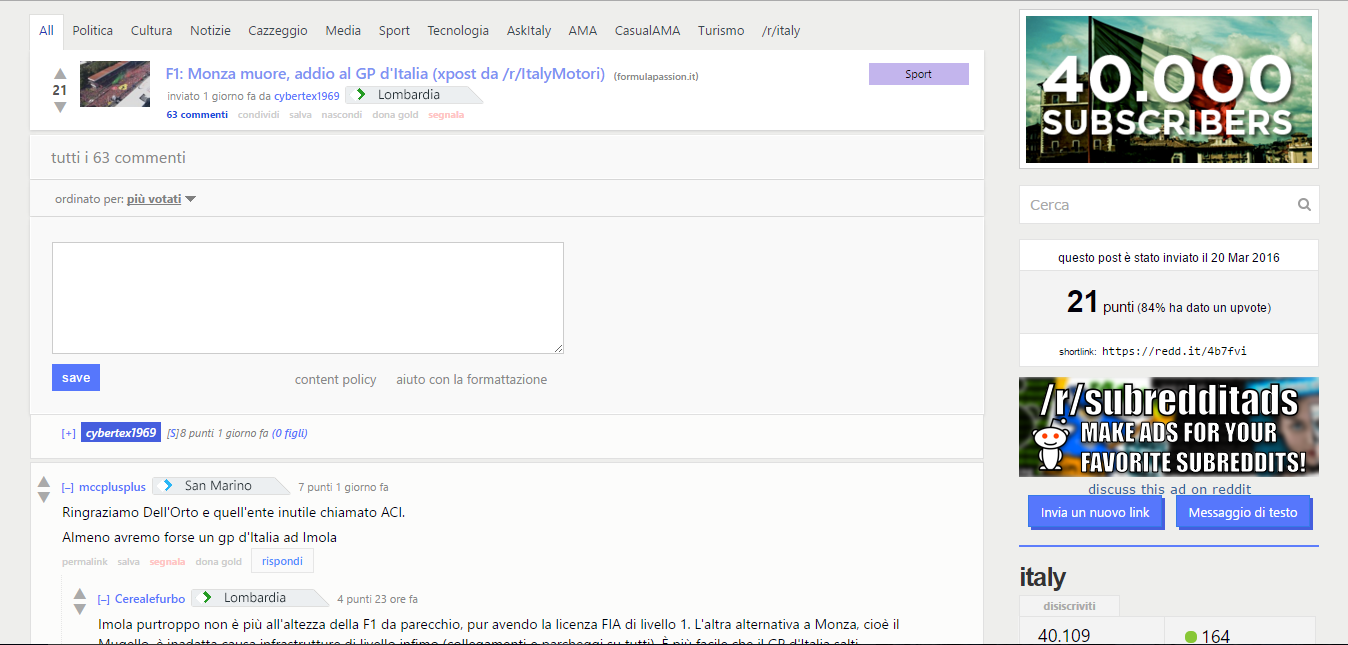
\includegraphics[width=90mm]{articolo}
\caption{vedi file articolo.png}
\end{figure}
\\
%manca sta parte da riguardare
Uno scomodo problema di Reddit consiste nell'assenza della possibilit\`a di accedere direttamente alla discussione relativa ad un contenuto (a meno che questo non sia un post puramente di testo) dall'interno del contenuto stesso: mi spiego con un esempio pratico. \\ \\L'utente sta navigando su /r/italy, vede il link "F1: Monza muore, addio al GP d'Italia", ci clicca e viene reindirizzato all'articolo di un sito esterno e fin qui tutto bene. In seguito alla lettura dell'articolo l'utente potrebbe essere interessato nel conoscere i pareri sull'argomento degli altri utenti di Reddit e qui sta la piccola "scomodit\`a":  per accedere alla discussione sull'argomento interna a Reddit l'utente deve ritornare alla pagina /r/italy su cui aveva trovato il link e cliccare sul "commenta" (scritto tra l'altro abbastanza in piccolo) appena sotto il link. \\Tutto questo andirivieni tra Reddit e siti esterni alla lunga pu\`o creare frustrazione nell'utente medio (che magari non pensa ad aprire il contenuto in una nuova scheda ma continua a navigare nella stessa causando il ricaricamento di pagine gi\`a visitate) e resta comunque poco pratico anche per l'utente esperto. \\ \\
Per quanto riguarda il sistema di commenti invece, la sua praticit\`a lo rende uno dei punti di forza del sito: i commenti sono strutturati "a cascata" dove ad ogni commento possono venire concatenati pi\`u commenti di risposta in maniera ricorsiva (un po' come if ed else annidati in C++). Detto cos\`i\ suona complicato ma \`e molto pi\`u semplice da vedere in pratica che da spiegare a parole (si veda ad esempio questa discussione - \url{https://redd.it/406d65}). \\ \\
La navigazione tra i commenti \`e davvero semplice, sono presenti metodi di sorting dei commenti in base al punteggio o alla data di pubblicazione e (tramite l'icona a "+" accanto al punteggio del commento) vi \`e la possibilit\`a di ridurre i commenti gi\`a letti passando cos\`i\ velocemente al successivo; alcune di queste funzionalit\`a avanzate richiedono un po' di tempo per acquisirne padronanza ma velocizzano enormemente il tempo di lettura di una discussione. \\ \\
Per quanto riguarda il form per la sottomissione di commenti (sia in risposta ad altri che a s\`e stanti) esso \`e semplicemente un rettangolo vuoto in cui inserire del testo, minimale ma intuitivo, in alcuni subreddit \`e inoltre presente un "tutorial" a scomparsa  per gli utenti che necessitano di funzionalit\`a  di scrittura pi\`u avanzate (ad es. testo con collegamento ipertestuale annesso oppure testo in grassetto ecc).

\section{Giudizio finale}
In conclusione, Reddit \`e una piattaforma all'apparenza complessa e dalle molteplici funzionalit\`a che possono spiazzare inizialmente i nuovi utenti ma al tempo stesso presenta una struttura efficiente e minimale dove l'utente che ha avuto il tempo di ambientarsi riesce a navigare con semplicit\`a.\\ \\ In base a tutti i punti esaminati durante questa analisi di usabilit\`a assegno a questo sito \textbf{7.5 punti su 10}.


\end{document}